\title{Assignment 5 -- CSC 225}
\author{
	Andrew \bf{Hobden} \\
	Student Number: \bf{V00788452}\\
	Instructor: Venkatesh Srinivasan
}
\date{\today}

\documentclass[12pt]{article}
\usepackage{mathtools}
\usepackage{amssymb}
\usepackage{algpseudocode}
\usepackage{algorithm}

\begin{document}
\maketitle

\section{Girth : Exercise 4.1.18, Page 559}
The {\bf girth} of a graph is the length of it's shortest cycle. If the graph is acyclic, then it's girth is infinite. Add a method {\bf girth()} to {\bf GraphProperties} that returns the girth of the graph. \\
Hint: Run BFS from each vertex. The shortest cycle containing $s$ is a shortest path from $s$ to some vertex $v$, plus the edge from $v$ back to $s$. \\
{\bf (Give pseudocode)} \\

\begin{algorithm}
\begin{algorithmic}[1]
	\Function{girth}{graph}
		\State result $\gets \infty$ 
		\Comment Size of the smallest cycle found
		\For{$vertex \in graph$}
			\State adjacents $\gets$ vertex.adjacentVertices()
			\State distance $\gets$ search(graph, vertex)
			\If{distance $\leq$ result}
				\State result $\gets$ distance
			\EndIf
		\EndFor
		\State \Return result
	\EndFunction
	
	\Function{search}{graph, source}
		\State queue $\gets$ new Queue
		\State queue.enqueue($source$)
		\State mark $source$
		\State distance(source) $\gets$ 0
		\State last $\gets$ source
		\Comment Store our last vertex.
		\While{Q is not empty}
			\State current $\gets$ Queue.dequeue()
			\For{neighbor in current.adjacentVertices()}
				\If{neighbor.marked() and neighbor is not last}
					\State \Return distance
					\Comment Found a cycle!
				\EndIf
				\State mark neighbor
				\State queue.enqueue(neighbor)
				\State distance(neighbor) $\gets$ distance(current)+1
			\EndFor
		\EndWhile
		\State \Return $\infty$
	\EndFunction
\end{algorithmic}
\end{algorithm}
\clearpage


\section{Odd Cycles : Exercise 4.1.33, Page 562}
Prove that a graph is two-colorable (bipartite) if and only if it contains no odd length cycle. \\
{\bf (Give a proof; try induction)} \\
\begin{center}
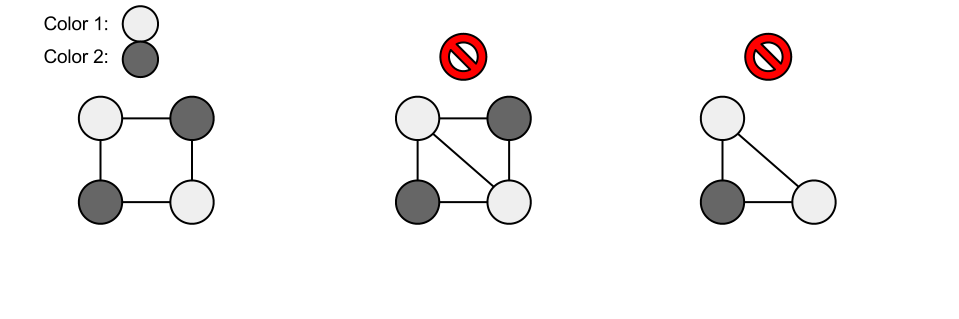
\includegraphics[width=0.8\textwidth]{figures/path.png}
\end{center}

\paragraph{Claim}
A graph $G$ is bipartite if and only if it contains no odd length cycle.

\subsection{Proof Part 1}
Proving a graph with odd cycles is never bipartite. \\
Consider the set of vertices forming an odd length cycle $\{v_1, v_2, v_3...,v_n\}$. In order for the graph to be bipartite each vertex must be a different color then it's neighbors, noting the first and last vertices are neighbors. We can assign $v_1(c_1)$ and $v_2(c_2)$, with every odd numbered vertex receiving $c_1$, and every even numbered vertex recieving $c_2$. Since $n$ is odd, $v_1$ \& $v_n$ must be colored both $c_1$, which is not compatible with the definition of bipartite. \\
Therefore, this is proven.

\subsection{Proof Part 2}
Proving a graph without odd cycles is always bipartite.
\paragraph{Base Case}
The smallest graph with no odd length cycles is an empty graph. This is trivially bipartite because there are no nodes which may not satisfy the parameters of bipartiteness.

\paragraph{Inductive Hypothesis}
Suppose that all graphs of size ${1, 2,..., n}$ without odd cycles are bipartite.

\paragraph{Inductive Step}
Consider a graph of size $n+1$ without odd cycles. \\
We can select any vertex $v$ from the graph, if is either not connected (thus not part of any cycle), connected to one vertex (still not part of any cycle), or connected to two vertices, which may be part of a cycle $C$. \\
Allow one vertex to be $X$ and one to be $Y$.
\begin{center}
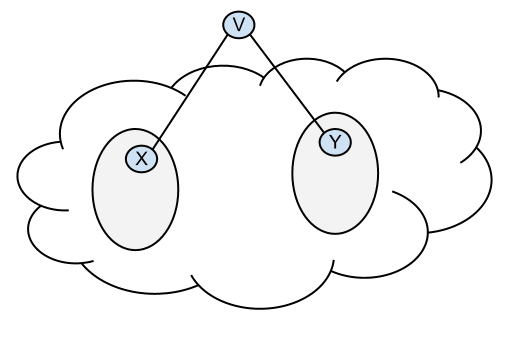
\includegraphics[width=0.8\textwidth]{figures/bipartite.png}
\end{center}
If there {\bf is not} odd path from $X$ to $Y$ in $G$, we simply move (recolor) $Y$ to be the same as $X$ and allow $V$ to assume the other color. \\
If there {\bf is} an odd path there is already a problem with the graph (see part 1.)

\paragraph{Conclusion} The claim holds.


\section{Exercise 4.2.12, Page 597}
How many edges are there in the transitive closure of a digraph that is a simple directed path with $V$ vertices and $V-1$ edges? \\
{\bf (Give a proof; try induction)} \\
\paragraph{Simple, directed path}
\begin{itemize}
	\item No parallel edges
	\item No multi-edges
	\item Directed
	\item Edges from $V_1$ to $V_2$ ... $V_2$ to $V_3$ ... $V_{n-1}$ to $V_n$
	\item No cycles
	\item One component
\end{itemize}

\paragraph{Thoughts}
From our definition we are guaranteed that $V_1$ will have a path to every future vertex. Thus, after the transitive closure it will have $V-1$ edges.
Each future vertex $V_n$, can be treated the same as $V_1$, allowing us to apply induction such that each $V_n$ will have $(V-n)-1$ edges.
\begin{center}
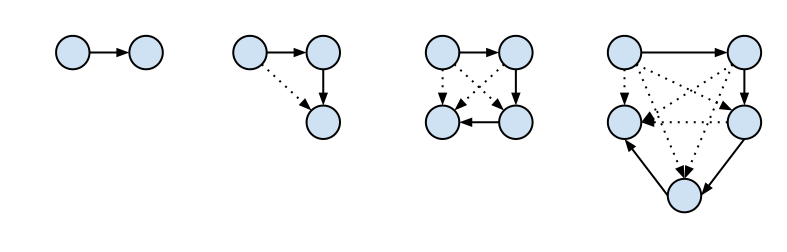
\includegraphics[width=\textwidth]{figures/closure.png}
\end{center}
\paragraph{Claim}
There are $\sum^{v}_{k=1} k-1$ edges in a transitive closure when applied to a simple directed path with $V$ vertices and $V-1$ edges when $V \geq 1$

\paragraph{Base Case}
Consider $V=1$ (Therefore $0$ edges). There are $0$ edges after a transitive closure, so the claim holds.

\paragraph{Inductive Hypothesis}
Suppose the claim holds for all $k \in {1,...,n}$.

\paragraph{Inductive Step}
Consider $n+1$. \\
We've added a new vertex along the path. It does not particularly matter where, since the resultant path is identical to if we just added a new vertex at the end.
	$$\sum^{n}_{k=1} (k-1) + (k+1)-1 = \sum^{n+1}_{k=1} (k-1)$$

Therefore, the claim holds for all $V \geq 1$.

\section{Unique Topological Ordering : Exercise 4.2.25, Page 598}
Design an algorithm to determine whether a digraph has a unique topological ordering. \\
Hint: A digraph has a unique topological ordering if and only if there is a directed edge between each pair of consecutive vertices in the topological order (i.e., the digraph has a Hamiltonian path). If the digraph has multiple topological orderings, then a second topological order can be obtained by swapping a pair of consecutive vertices.

\paragraph{Disclaimer}
Bill Bird explicitly stated in class that code was not a requirement, therefore it has been left out for the sake of simplicity.
% TODO -- Allowed to assume you have topological sorting at disposal. Don't have to give code, just describe.
\paragraph{Steps}
\begin{itemize}
	\item Topological Sort the graph $G$.
	\item Check for a hamiltonian path of the sorted graph.
	\item If a path is found, then the digraph's topological sort is unique.
	\item If a path is not found, then the sort is not unique.
\end{itemize}

\section{Exercise 4.3.3, Page 631}
Show that if a graph's edges all have distinct weights, the MST is unique. \\
{\bf (Give a proof; try contradiction)} \\

\subsection{Proof by Contradiction}
Suppose a graph with all distinct weights has two MSTs. We'll call them $G$ and $F$.
$$ G = g_1 < g_2 < ... < g_i < ... < g_n $$
$$ F = f_1 < f_2 < ... < f_i < ... < f_n $$
If possible, let $F$ and $G$ be not identical. \\
We can iterate through the MST until we find an $i$ such that $f_i \neq g_i$ which implies further that $weight(f_i) \neq weight(g_i)$, since all weights are distinct.
Therefore, there are two cases:
\subsubsection{Case 1: $weight(g_i) < weight(f_i)$}
Since $g_i$ is distinct from $ \{f_1, f_2, ..., f_{i-1} \} $ and it is not after $f_i$ since $weight(g_i) < weight(f_i)$ we shall add $g_i$ to the spanning tree $F$. This creates a cycle $c$ in the MST which has one of two cases:
\begin{itemize}
	\item $g_i$ is not the heaviest edge in $c$, therefore there is a better graph for $F$. This resultant tree is either identical to $G$ or can be found to be by repeating this proof as many times are needed such that for all $g_a = f_a$.
	\item $g_i$ is the heaviest edge in $c$. This means that $\{g_i\}\cup\{f_1, f_2, ...,f_{i-1}\}$ must contain a cycle. However this also implies (since $F$ and $G$ were equal up to $i-1$) that $\{g_i\}\cup\{g_1, g_2, ...,g_{i-1}\}$ also contains a cycle, which is not allowed.
\end{itemize}

\subsubsection{Case 2: $weight(g_i) > weight(f_i)$}
The list of vertices must have looked like $\{g_1, g_2, ... , f_i, g_i, ...\}$. However, $f_i$ was not chosen by the MST algorithm, which implies that $\{f_i\} \cup \{g_1, g_2, ..., g_i\}$ contains a cycle. Since this means that $F$ contains a cycle, this is not possible. \\
What if $i<2$? This is not possible either, since there would be no cycles formed by $f_i$ as there are not enough edges. So the MST algorithm would have picked $f_i$, but this is a contradiction.

\paragraph{Conclusion}
Therefore, $f_i = g_i$, so the trees are identical, thus the single tree is unique.

\section{Exercise 4.3.7, Page 631}
How would you find a {\bf maximum} spanning tree of an edge weighted graph?

\paragraph{Solution}
You could simply use the Prim-Jarnik-Dijkstra (or Kruskel's) algorithm, and instead of selecting the smallest weighted edge just select the largest weighted edge. Correctness could be proven via using the Cut Property (If using Prim-Jarnik-Dijkstra.)


\end{document}